\part{Advanced C-Fu}\toc
%%%%%%%%%%%%%%%%%%%%%%%%%%%%%%%%%%%%%%%%%%%%%%%%%%%%%%%%%%%%%%%%%%%%%%%%%%%%%%%
\section{Modular C}
\subsection{Organizing large C projects}
\begin{frame}[fragile]{Organizing large C projects}
  \vspace{-1.2\baselineskip}
  \begin{block}{}
    \begin{itemize} 
    \item You are free in C: many ways to organize your code, nothing is enforced
    \item Get organized by yourself, or you'll get drown in your own code
    \end{itemize}
  \end{block}\vspace{-.5\baselineskip}

  \begin{block}{Guidelines for Java programmers in C %
      {\normalsize(Light and DIY object-orientation)}}
    \begin{itemize}
    \item Organize your code as several interacting classes
    \item Avoid inheritance by all means: ugly to mimick in C, often not helping
      anyway
    \item You can still get encapsulating and some of dynamic dispatch
    \item Each class becomes a module:
      \begin{itemize}
      \item A structure, grouping all fields of your class
      \item A set of functions acting on those structures (incl. constructor \&
        destructor)
      \end{itemize}
    \item Nothing is enforced; your code should remain clean %
      {\small(and your days pleasant)}
      \begin{itemize}
      \item Code readability as main objective (you are the main reader, help
        the reader)
      \end{itemize}
    \end{itemize}
  \end{block}

  \begin{block}{Forget about the performance, genericity, reusability \ldots~
      for now}
    
  \end{block}\vspace{-\baselineskip}
  \begin{quote}{}
    % Programmers waste enormous amounts of time thinking about, or worrying
    % about, the speed of noncritical parts of their programs, and these attempts
    % at efficiency actually have a strong negative impact when debugging and
    % maintenance are considered. 
    We should forget about small efficiencies, say about 97\% of the time:
    {\bf premature optimization is the root of all evil}. Yet we should not pass up
    our opportunities in that critical 3\%. \hfill{\rm --- Donald Knuth}
  \end{quote}
\end{frame}
%%%%%%%%%%%%%%%%%%%%%%%%%%%%%%%%%%%%%%%%%%%%%%%%%%%%
\begin{frame}[fragile]{The \texttt{point} module}

  \begin{block}{Changing each class into a module}
    \begin{itemize}
    \item A structure, grouping all fields of your class
    \item A set of functions acting on those structures (incl. constructor \&
      destructor)
    \end{itemize}
  \end{block}

  \begin{columns}
    \begin{column}{.25\linewidth}
      \begin{boitecode}{}
typedef struct \{
  int x, y;
\} point_t;              
      \end{boitecode}
    \end{column}
    \begin{column}{.6\linewidth}
      \begin{boitecode}{}
point_t *point_create(int x, int y);
void point_free(point_t *p);

void point_move(point_t *p, int dx, int dy);      
void point_add(point_t *p1, point_t *p2);      
      \end{boitecode}
    \end{column}
  \end{columns}

  \begin{center}
    \begin{tabular}{|l|l|}\hline
      \multicolumn{1}{|c|}{\structure{Java}}&\multicolumn{1}{c|}{\structure{C}}\\\hline
      References to objects&Pointers to structures\\\hline
      
      Methods included in object& Functions grouped by modules\\
      & Naming conventions at best\\\hline
      
      Dotted notation&Receiver as first parameter\\
      \multicolumn{1}{|c|}{\texttt{p.move(3,5)}}& 
      \multicolumn{1}{c|}{\texttt{point\_move(p, 3,5)}}\\\hline
      
      Automatic garbage collection&Manual memory handling\\\hline
    \end{tabular}
  \end{center}
\end{frame}

%%%%%%%%%%%%%%%%%%%%%%%%%%%%%%%%%%%%%%%%%%%%%%%%%%%%
\begin{frame}[fragile]{Full code of the \texttt{point} module}
  \begin{columns}
    \begin{column}{.45\linewidth}
      \begin{boitecode}{}
typedef struct \{
  int x, y;
\} point_t;              
      \end{boitecode}

      \begin{boitecode}{point\_t *{\bf point\_create}(int x, int y) \{}
  point_t *res=malloc(sizeof(point_t));
  res->x = x;
  res->y = y;
  return res;
\}
      \end{boitecode}

      \medskip
      \begin{boitecode}{void {\bf point\_free}(point\_t *p) \{}
  free(p);// plz still use a free function: 
\}         // more extensible for future
      \end{boitecode}
    \end{column}
    \begin{column}{.45\linewidth}
      \begin{boitecode}{void {\bf point\_move}(point\_t *p,\\
          \null~~~~~~~~~~~~~~~~~~~~~~ int dx, int dy) \{}
  p->x += dx; // p->x shortcut of (*p).x
  p->y += dy;
\}
      \end{boitecode}
      \medskip
      \begin{boitecode}{void {\bf point\_add}(point\_t *p1,\\
          \null~~~~~~~~~~~~~~~~~~~~point\_t *p2) \{}
  p1->x += p2->x;
  p1->y += p2->y;
\}
      \end{boitecode}
  \end{column}
  \end{columns}

  \begin{itemize}
  \item This really feels as Java, and this is a good news:
  \item You can code in C and still organize your code as you've learned

    \bigskip
  \item Missing: Hiding the implementation: How to have private methods and fields?
  \item Missing: Dynamic dispatch. Functions' pointers can simulate this.
  \item Missing: Inheritance. No easy way (but several ugly ones ;)
  \end{itemize}
\end{frame}
%%%%%%%%%%%%%%%%%%%%%%%%%%%%%%%%%%%%%%%%%%%%%%%%%%%%
\begin{frame}[fragile]{Having private methods in C modules}
  \begin{block}{The File is the Compilation Unit}
    \begin{itemize}
    \item Hidden methods must simply be marked \alert{\texttt{static}} $\Rightarrow$
      visible from that file only
    \item This older habit explains why Java forces public classes to have their
      own file
    \end{itemize}
  \end{block}

  \begin{block}{How to make parts visible from outside? With \structure{\textbf{header files}}!}
    \begin{itemize}
    \item Regular C files named \framebox{\texttt{point.\alert{h}}} containing
      structures \& function prototypes
    \item Hide your implementation $\Rightarrow$ hide the struct's content
      (\structure{\textbf{opaque structure}})
    \end{itemize}
  \end{block}

  \begin{columns}
    \begin{column}{.47\linewidth}
      \begin{boitecode}{point.h}
typedef struct point point_t;              

point_t *point_create(int x, int y);
void point_free(point_t *p);

void point_move(point_t *p, int dx, int dy);      
void point_add(point_t *p1, point_t *p2);      
      \end{boitecode}
    \end{column}

    \begin{column}{.45\linewidth}
      \begin{boitecode}{point.c}
\#include "point.h"
struct point \{
  int x,y;
\};

point_t *point_create(int x, int y) \{
  point_t *res = malloc(sizeof(point_t));
  res->x = x;
  res->y = y;
  return res;
\} 
      ...
      \end{boitecode}
    \end{column}
  \end{columns}
\end{frame}
%%%%%%%%%%%%%%%%%%%%%%%%%%%%%%%%%%%%%%%%%%%%%
\begin{frame}[fragile]{Dealing with the compiler's stupidity}
  \begin{block}{Problem: the C compiler is really prehistoric}
    \begin{itemize}
    \item Complains when symbols get redefined (even if the
      definitions match)
    \item Problem when \texttt{point.h} $\in$ \texttt{square.h} $\in$
      \texttt{main.c} and \texttt{square.h} $\in$ \texttt{main.c}
    \item \structure{\textbf{Multiple inclusion}} of \texttt{point.h} into
      \texttt{main.c}, leading to compilation error
    \end{itemize}
  \end{block}

  \begin{block}{Solution: fix the code before compiling}
    \begin{itemize}
    \item Remember: the preprocessor changes the code presented to the compiler
    \item We need to hide the subsequent inclusions of files
    \end{itemize}
  \end{block}

  \begin{columns}
    \begin{column}{.47\linewidth}
      \begin{boitecode}{point.h}
\alert{\textbf{\#ifndef POINT\_H}}
\alert{\textbf{\#define POINT\_H}}
typedef struct point point_t;              

point_t *point_create(int x, int y);
void point_free(point_t *p);

void point_move(point_t *p, int dx, int dy);      
void point_add(point_t *p1, point_t *p2);      
\alert{\textbf{\#endif /* POINT\_H */}}
      \end{boitecode}
    \end{column}

    \begin{column}{.48\linewidth}
      \begin{itemize}\vspace{-.6\baselineskip}
      \item \texttt{point.c} remains unchanged
      \item This construct seems ugly first
      \item But this is the one true way
      \item Just works, simple and efficient
      \item Not sufficient on Windows.\\
        C on Windows is pure masochism\\
        (but not because of C)
      \end{itemize}
    \end{column}
  \end{columns}
\end{frame}
%%%%%%%%%%%%%%%%%%%%%%%%%%%%%%%%%%%%%%%%%%%%%
\begin{frame}[fragile,squeeze]{Advanced OOP in C}
  \begin{block}{Dynamic dispatch}
    \begin{itemize}
    \item Structures can contain pointers to function (but shouldn't when possible)
    \end{itemize}
    \begin{columns}
      \begin{column}{.5\linewidth}
        \begin{boitecode}{}
typedef struct point *point_t; // forward decl
struct point \{
  int x, y;
  void \alert{(*display)}(point_t* p);
\} 
        \end{boitecode}
      \end{column}
      \begin{column}{.39\linewidth}
        \begin{boitecode}{}
void my_display(point_t*p) \{..\}
     ...
p1->display = &my\_display;          
     ...
(*(p1->display)) (p1); // just a call
        \end{boitecode}
      \end{column}
    \end{columns}
  \end{block}\vspace{-.3\baselineskip}

  \begin{block}{Inheritance}
    \begin{itemize}
    \item Including structures is a UGLY but working approach. \alert{Don't do
        this for real}
    \item Inheritance is over-sold anyway. You should never expose your
      inheritance tree
    \end{itemize}

    \begin{columns}
      \begin{column}{.5\linewidth}
        \begin{boitecode}{}
typedef struct particle \{
  point_t super; // whole structure copied over
  int vx, vy;
\} particle_t;
        \end{boitecode}
      \end{column}
      \begin{column}{.39\linewidth}
        \begin{boitecode}{}
void particle_animate(particle_t *mp) \{
  mp->super.x = p1->vx;
  mp->super.y = p1->vy;
\}
        \end{boitecode}
      \end{column}
    \end{columns}\vspace{-.5\baselineskip}
    \begin{itemize}
    \item Any particle can even be casted into a point to retrieve x and y
    \item But NO SAFEGUARD here. So pain to debug, impossible to read, etc.
    \item Y U NO C++ (or Objective C) if you really need OOP in C??
    \end{itemize}

  \end{block}
\end{frame}
%%%%%%%%%%%%%%%%%%%%%%%%%%%%%%%%%%%%%%%%%%%%%
\subsection{Compiling Multi-Files Projects and Makefiles}
\begin{frame}{Having many files in your project (one per module)}
  \begin{block}{That's a good habit}
    \begin{itemize}
    \item Because a 500,000 lines file is hard to navigate 
    \item Because  we can compile each of them separately
      \begin{itemize}
      \item Remember: compilation = translation into assembly lang. + linking of ASM
      \item Translation: hard and takes time; Assembling the puzzle: much faster
      \item Multiple files allows to translate only the parts that changed
      \end{itemize}
    \item Because several people can work on the same project w/o interfering
    \end{itemize}
  \end{block}\vspace{-.5\baselineskip}
  \begin{block}<2->{But harder to compile right}
    \begin{itemize}
    \item \structure{Compilation:} 
      \fbox{\small\texttt{gcc -c point.c}} 
      \fbox{\small\texttt{gcc -c square.c}} 
      \fbox{\small\texttt{gcc -c main.c}}\\[2pt]
      {\small It generates \texttt{point.o, square.o, main.o} containing the
        assembly translations}
    \item \structure{Linking:} 
      \fbox{\small\texttt{gcc -o project point.o square.o main.o}}
    \item Tracking dependencies is a nightmare \textit{e.g.} when header files
      are changed
    \item We need a specific tool for that\visible<3>{. It's called
        \structure{\textbf{make}}}
    \item<3> Even from eclipse, use makefiles. Obey the UNIX philosophy:

      \smallskip \centerline{\it Write programs that do one thing and do it
        well. Write programs to work together.}
  \end{itemize}
  \end{block}
\end{frame}

%%%%%%%%%%%%%%%%%%%%%%%%%%%%%%%%%%%%%%%%%%%%%%%%%%%%%%%%%%%%%%%%%%%%%%%%%%%%%%%
\begin{frame}[fragile]{Make and Makefiles}
  \begin{block}{Makefile: explaining the project building process}    
    \begin{itemize}
    \item Create a file named \framebox{\texttt{Makefile}} in your project,
      containing a set of rules
        {  \footnotesize
        \begin{semiverbatim}
<target file>: <list of dependencies>
    <command to build target from deps>
        \end{semiverbatim}}\vspace{-.7\baselineskip}
    \end{itemize}
  \begin{columns}
    \begin{column}{.45\linewidth}\medskip
  \begin{boitecode}{Simple Makefile}
project: point.o square.o main.o
    gcc point.o square.o main.o -o project

point.o: point.c point.h
    gcc -c point.c

square.o: square.c square.h point.h
    gcc -c square.c

main.o: main.c square.h point.h
    gcc -c main.c
  \end{boitecode}      
    \end{column}
    \begin{column}{.48\linewidth}
      \begin{boitecode}{\texttt{make} already knows to build .o from .c}
project: point.o square.o main.o
    gcc point.o square.o main.o -o project

point.o: point.c point.h
square.o: square.c square.h point.h
main.o: main.c square.h point.h
      \end{boitecode}

      \vspace{-.7\baselineskip}
      \begin{boitecode}{\texttt{make} loves funky variable names}
project: point.o square.o main.o
    gcc \$^ -o \$@
      \end{boitecode}
    \end{column}
  \end{columns}
  \end{block}
  \begin{itemize}\vspace{-.2\baselineskip}
  \item Builds first target by default; Specify another one if you want
    \framebox{\texttt{make clean}}
  \item\texttt{make} is used widely, not only for C. You could use it for you Java code!
  \end{itemize}
\end{frame}

%%%%%%%%%%%%%%%%%%%%%%%%%%%%%%%%%%
\section{The Many Ways of Messing Up in C}\subtoc
\subsection{Syntax Pitfalls}
\begin{frame}{}
  \thispagestyle{empty}
  \begin{center}
    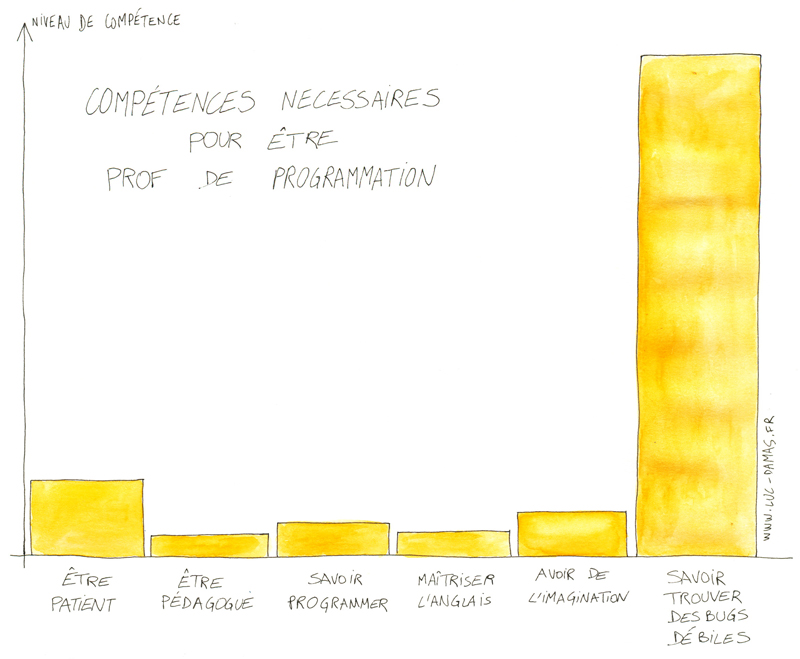
\includegraphics[width=.9\linewidth]{img/competences-prof-programmation.jpg}
    %
    \rotatebox{90}{~~~~~~~~~~~~~~~~~~~~
\includegraphics[width=7mm]{img/by-nc-sa.png}}
  \end{center}
\end{frame}

%%%%%%%%%%%%%%%%%%%%%%%%%%%%%%%%%%
\begin{frame}[fragile,squeeze]{Classical errors with the \texttt{for} loop}
  \begin{columns}
    \begin{column}{.35\linewidth}
      \begin{boitecode}{}
for (i=0; i < 10; \alert<2>{i+1})
   printf("i=\%d\n",i);
      \end{boitecode}
    \end{column}

    \begin{column}<2->{.6\linewidth}
      \begin{itemize}\vspace{-1.3\baselineskip}
      \item Y U NO increment your counter??
      \item[] (\texttt{i+1} has no side effect)
      \end{itemize}
    \end{column}
  \end{columns}

  \begin{columns}
    \begin{column}<2->{.35\linewidth}
      \begin{boitecode}{}
for (i=0; \alert<3>{i = 10}; i++) 
   printf("i=\%d\n",i);
      \end{boitecode}
    \end{column}

    \begin{column}<3->{.6\linewidth}
      \begin{itemize}\vspace{-1.3\baselineskip}
      \item Y U NO test your counter??
      \item[] (\texttt{i=10} sets a new value)
      \end{itemize}
    \end{column}
  \end{columns} 

  \begin{columns}
    \begin{column}<3->{.35\linewidth}
      \begin{boitecode}{}
for (i=0; i < 10; i++)\alert<4>{;}
   printf("i=\%d\n",i);
      \end{boitecode}
    \end{column}

    \begin{column}<4->{.6\linewidth}
      \begin{itemize}\vspace{-1.3\baselineskip}
      \item Y U NO enter your loop??
      \item[] (the \framebox{;} after the \texttt{for} closes the loop)
      \end{itemize}
    \end{column}
  \end{columns}

  \begin{columns}
    \begin{column}<4->{.35\linewidth}
      \begin{boitecode}{}
for (\alert<5>{i=0, j=0}; i < 10; i++)
   printf("i=\%d\n",i);
      \end{boitecode}
    \end{column}

    \begin{column}<5->{.6\linewidth}
      \begin{itemize}\vspace{-1.3\baselineskip}
      \item Y U NO see when it's correct??
      \item[] \framebox{,} separate expressions, \framebox{;} instructions
      \end{itemize}
    \end{column}
  \end{columns}
\end{frame}

%%%%%%%%%%%%%%%%%%%%%%%%%%
\begin{frame}[fragile]{Beware of the vicious \texttt{switch} syntax!}
  \begin{columns}
    \begin{column}{.23\linewidth}
      \begin{boitecode}{}
int x = 2;
switch(x) \{
  case 2:
    printf("Two\n");
  case 3:
    printf("Three\n");
\}     
      \end{boitecode}
    \end{column}
    \begin{column}<2->{.6\linewidth}
      \begin{itemize}
      \item Prints both: \framebox{\hbox to .32\linewidth{\vbox{\texttt{Two\\Three}}}}
      \item Problem: missing \texttt{break} keywords
      \item Because in assembly, that's a jump table
      \end{itemize}
    \end{column}
  \end{columns}

  \visible<2->{
    \begin{itemize}
    \item So that's a (sad) inheritance of assembly language
    \item And that's very sad that this propagated to Java\ldots
    \item This also explains why \texttt{case} values must be constant
    \end{itemize}
  }
\end{frame}
%%%%%%%%%%%%%%%%%%%%%%%%%%

\subsection{Understanding gcc Error Messages}
\begin{frame}[fragile]{Understanding \texttt{gcc} error messages}
  \centerline{\texttt{gcc} \textbf{is} user friendly. It's just picky about its
    friends}\smallskip
  \concept{But you \textbf{have to} pass \framebox{\texttt{-Wall -Wextra}} as parameter}

   \bigskip
   \bigskip

  \begin{block}{Suggest parentheses around assignment used as truth value\ldots}
    \bigskip\smallskip
    \begin{columns}
      \begin{column}{.1\linewidth}
        \begin{boitecode}{}
if (a=b)
        \end{boitecode}
      \end{column}
      \begin{column}<2>{.78\linewidth}
        \begin{itemize}\vspace{-1.3\baselineskip}
        \item \ldots if you \textbf{really} mean to erase a, 
          then write \framebox{if ((a=b))}
        \item Else, you probably meant \framebox{if (a==b)}
        \item The compiler gives a meaning even to the weird \framebox{if ((a=b)!=0)}
        \end{itemize}
      \end{column}
    \end{columns}
  \end{block}
\end{frame}
%%%%%%%%%%%%%%%%%%%%%%%%%%%%%%%%%%%
\begin{frame}[fragile]{Return of functions}
  \begin{itemize}
  \item \structure{\large warning: 'return' with a value, in function returning void}\\
    Yeah that's only a warning --- keep calm and add \framebox{\texttt{-Werror}}
    

    \bigskip
  \item<2-> \structure{\large Control reaches end of non void function:} self
    explanatory (?)
  \end{itemize}

  \begin{columns}
    \begin{column}<2->{.3\linewidth}
      \begin{boitecode}{\alert{\bf Don't do that}}
int my_function() \{
   if (x == 2)
      return 1;
\}

      \end{boitecode}
    \end{column}
    \begin{column}<3->{.28\linewidth}
      \begin{boitecode}{This is correct}
int my_function() \{
   if (x == 2)
      return 1;
   \alert<3>{return 0;}
\}
      \end{boitecode}
    \end{column}
    \begin{column}<3->{.28\linewidth}
      \begin{boitecode}{This is correct too}
\alert<3>{void} my_function() \{
   if (x == 2)
      printf("blah");
\}

      \end{boitecode}
    \end{column}
  \end{columns}

\end{frame}
%%%%%%%%%%%%%%%%%%%%%%%%%%%%%%%%%%%
\begin{frame}[fragile]{Declarations}
  \begin{block}{Implicit declaration of function func}
    \begin{itemize}
    \item The function was used before being declared
    \item Just warning; the creepy compiler assumes "no parameter, returning integer"
%       \begin{columns}
%         \begin{column}{.7\linewidth}
%           \begin{boitecode}{}
% int func() \{...\}        


% \end{boitecode}
%         \end{column}
%       \end{columns}
    \item If you declare the function \textbf{after} its use, the message reads:
      \begin{itemize}
      \item[] \structure{\large warning: conflicting types for 'func'}
      \item and you are informed of where the "declaring usage" occured
      \end{itemize}
    \end{itemize}
  \end{block}

  \begin{block}{Too few/many arguments to function}
    \begin{itemize}
    \item Good programmers have a rare ability: they \textit{try} to read error
      messages!
    \end{itemize}
  \end{block}

  \begin{block}{Passing arg n of func from incompatible pointer type}
    \begin{itemize}
    \item Seems innocuous, but often denotes (upcoming) subtle issue
    \end{itemize}
  \end{block}

  \begin{block}{Passing arg n of func makes pointer from integer without a cast}
    \begin{itemize}
    \item The numerical value of pointers should not be messed with as in 

      \framebox{\hbox to .42\linewidth{\vbox{\small\texttt{int value=42;\\int length=strlen(value);}}}}
    \end{itemize}
  \end{block}
\end{frame}
%%%%%%%%%%%%%%%%%%
\subsection{Messing Up With Memory}
\begin{frame}[fragile]{Messing Up With Memory}
  \begin{columns}
    \begin{column}{.4\linewidth}
  \begin{boitecode}{}
#include <stdio.h>
#include <stdlib.h>
#include <string.h>
int main(int argc, char *argv[]) \{
  char *truc = "constant string";
  *truc = 'x';          \alert{// segfault}
  strcpy(truc, "toto"); \alert{// segfault}
  free(truc);           \alert{// segfault}
  return 0;
\}
  \end{boitecode}    
 
  \begin{boitecode}{}
  int i = 42;
  printf("%s",i); \alert{// invalid read}
  \end{boitecode}
    \end{column}
    \begin{column}{.46\linewidth}
      \begin{boitecode}{}
int *make_buff(int a) \{
  int buff[SIZE], cpt;
  for (cpt=0; cpt<SIZE; cpt++) 
    buff[cpt] = a;
  return buff; \alert{// pointer to invalid memory}
\}
      \end{boitecode}

      \begin{boitecode}{}
  char *buffer;
  scanf("%s", buffer); \alert{// invalid write}
      \end{boitecode}
      \bigskip

      \begin{boitecode}{}
  char buffer[256];      \alert{// constants }
  for (i=0; i<1024; i++) \alert{//   shouldn't}
     buffer[i] = ' ';    \alert{//     change}
      \end{boitecode}
    \end{column}
\end{columns}

  \bigskip
  \bigskip
  \bigskip
  \concept{But this aint fun: messing up with pointers is too easy}

  \centerline{we'll see in practical how to hunt down these issues with valgrind}
\end{frame}
%%%%%%%%%%%%%%%%%%%%%%%%%%%%%%%%%%%%%%%%
% \section{Development tools for C}\subtoc
% \subsection{Detecting Memory Errors}
% \begin{frame}{Detecting Memory Errors}
%   \begin{block}
    
%   \end{block}
% \end{frame}

%%%%%%%%%%%%%%%%%%%%%%%%%%%%%%%%%%%%%%%%
\section{Doing a Game in C}\subtoc
\begin{frame}{Doing a game in C}
  \begin{block}{Mandatory elements}
    \begin{itemize}
    \item \structure{A gameplay:} an idea about what your game will be
    \item \structure{A game engine:} a program that can interact with the player
    \item \structure{Some GFX:} graphics, sounds, musics, etc.
    \item These may not suffice for a great game, but at least they are mandatory
    \end{itemize}
  \end{block}\vspace{-.5\baselineskip}

  \begin{block}{Where to find the inspiration for your gameplay}
    \begin{itemize}
    \item Kongregate, play.google.com or whatever.
    \item Many links on \url{http://www.loria.fr/~quinson/Hacking/Curiosa/}
    \end{itemize}
  \end{block}\vspace{-.5\baselineskip}

  \begin{block}{Doing a game engine}
    \begin{itemize}
    \item It's actually  easy (with SDL2, SFML or allegro)! %
      \textbf{That's your assignment}
    \item See \url{http://www.loria.fr/~vthomas/enseignement/2013_JV_ESIAL/}
    \end{itemize}
  \end{block}\vspace{-.5\baselineskip}

  \begin{block}{Finding some GFX}
    \begin{itemize}
    \item That's \textbf{not} your assignment. It's sufficient to find something online
    \item But please don't \textit{steal} your GFX. Free resources exist.
    \end{itemize}
  \end{block}
\end{frame}
%%%%%%%%%%%%%%%%%%%%%%%%%%%%%%%%%%%%%%%%%%%%%%%
\begin{frame}{Logistics of the project}
  \begin{itemize}
  \item \structure{Groups:} 2 or 3 peoples (not 1, not 4). You can mix classes
  \item \structure{When:} first week empty of lectures at Telecom Nancy
    ($\approx$ end May)
  \item \structure{What:} discuss per email with me so that we agree on an assignment
  \item \structure{How long:} don't assume you can do something in 2 weeks only
  \item \structure{Other constraints:}
    \begin{itemize}
    \item Must be in C (or C++ if good reasons), under Linux (C is
      \textbf{NOT} portable)
    \item Must be rather original \& involve some coding %
      {\small(no mastermind/memory please)}
    \item Should induce a graphical interface, may contain an AI
    \item That's very open: do what you would like to (one-time offer in your scholarship)
    \end{itemize}
  \item \structure{What gets evaluated:} report (5 pages max) + source code + oral defense
    \begin{itemize}
    \item A short public presentation: 10 lines description + screenshot +
      licensing info
    \item List of issues encountered and your solutions (no code!)
    \item Approximate amount of time spent per student and per task
    \item Exhaustive list of source of informations you've used 
    \end{itemize}
  \item   You \textbf{must} get my approval before starting.
    \begin{itemize}
    \item Try talking to me after my teachings if I don't answer my emails in time
    \item Don't wait the week before the defenses or I'll know ;)
    \end{itemize}
  \end{itemize}
\end{frame}